% !Mode:: "TeX:UTF-8"
% !TEX builder = LATEXMK
% !TEX program = xelatex
\documentclass[master,oneside,AutoFakeBold]{zjuthesis} % 如果你的论文不满80页,还是单面印刷吧


%%%%%%%%%%%%%%%%%%%%%%%%%%%%%% 开始填写前置部分使用的变量
%%%%%%%%%%%%%%%%%%%%%%%%%%%%%% 样式设定在 zjuthesis.cls 下, 人类可读,爱请查阅

% 这里写这么鬼畜是为了测试多几个字会不会造成溢出
\title{某某某某某科学的浙江大学软件学院硕士论文模板} % 封面和题名页使用
\englishtitle{Toaru Kagaku no Template of Software Engineering Thesis in \LaTeX } % 封面和题名页使用
% 如果您的标题用字过多,请自行调节 zjuthesis.cls 里的 ZJUmakecover 里的各项距离。

%\author{伊藤春希}          % 申请人姓名 封面使用
\author{王宝华}

\classification{TP311.5}    % 封面头使用
\serialnumber{10335}        % 封面头使用
\secretlevel{无}            % 封面头使用
\studentnumber{21x51xxx}    % 封面头使用

%\supervisor{御坂美琴}       % 导师 封面使用
\supervisor{干红华}
%\spvtitle{电击使}           % 职称 封面使用
\spvtitle{副教授}              % 职称 封面使用

%\cpsupervisor{桂和纱}       % 合作导师,如果没有合作导师,就在此文件第 4 行\documentclass选项栏中加上"nocpsupervisor"。
\cpsupervisor{师之名}
\cspvtitle{职称}             % 合作导师职称

% 从机械工程学院改来,保留设定变量命名
%\major{船舶工程}            % 专业学位类别栏 填 工程硕士
\major{工程硕士}
%\research{白学}             % 专业学位领域栏 填 软件工程
\research{软件工程}
\institute{软件学院}         % 所在学位栏 填 软件学院

\submitdate{2022年12月20日}   % 论文提交日期 栏

% 题名页的评阅人及答辩席
% 归档时候填写
% 论文评阅人1 2 3 4 5
\reviewerA{} \enreviewerA{}
\reviewerB{} \enreviewerB{}
\reviewerC{} \enreviewerC{}
\reviewerD{} \enreviewerD{}
\reviewerE{} \enreviewerE{}

% 答辩委员会主席
\chairperson{} \enchairperson{}

% 答辩委员 1 2 3 4 5
\commissionerA{} \encommissionerA{}
\commissionerB{} \encommissionerB{}
\commissionerC{} \encommissionerC{}
\commissionerD{} \encommissionerD{}
\commissionerE{} \encommissionerE{}

% 答辩日期
\defencedate{2022年12月26日} \eendefencedate{}  % 因为endefencedate 命名被占用

% 论文前置部分变量填写完毕 开始全书排版
\begin{document}

% 封面、中文题名页、英文题名页、独创声明和版权使用书 无页码
\maketitle

% 摘要部分
\abstractmatter
% !TEX root = ../main.tex

% 定义中文摘要和关键字
\begin{cabstract}
请注意,以下内容主要参考自薛瑞尼的清华大学论文模板。

论文的摘要是对论文研究内容和成果的高度概括。
摘要应对论文所研究的问题及其研究\textbf{目的}进行描述,
对研究\textbf{方法和过程}进行简单介绍,
对研究\textbf{成果和所得结论}进行概括。
摘要应具有独立性和自明性,
其内容应包含与论文全文等量的主要信息。
使读者即使不阅读全文,
通过摘要就能了解论文的总体内容和主要成果。

论文摘要的书写应力求精确、简明。切忌写成对论文书写内容进行提要的形式,尤其要避
免“第 1 章……;第 2 章……;……”这种或类似的陈述方式。
不宜使用公式、图表,不标注引用文献。
硕士论文摘要的字数一般为300--500 个左右。

关键词是为了文献标引工作、
用以表示全文主要内容信息的单词或术语。
关键词不超过 5个,
每个关键词中间用分号分隔
(研究生院要求使用分号分隔,软件学院要求使用逗号分隔)。
见源码\texttt{zjuthesis.cls}搜索keywords了解。
\end{cabstract}

\ckeywords{\LaTeX, CJK, 模板, 毕业论文}

% !TEX root = ../main.tex

% 定义英文摘要和关键字

\begin{eabstract}
An abstract of a dissertation is a summary and extraction of research work
and contributions. Included in an abstract should be description of research
topic and research objective, brief introduction to methodology and research
process, and summarization of conclusion and contributions of the
research. An abstract should be characterized by independence and clarity and
carry identical information with the dissertation. It should be such that the
general idea and major contributions of the dissertation are conveyed without
reading the dissertation.

An abstract should be concise and to the point. It is a misunderstanding to
make an abstract an outline of the dissertation and words ``the first
chapter'', ``the second chapter'' and the like should be avoided in the
abstract.

Key words are terms used in a dissertation for indexing, reflecting core
information of the dissertation. An abstract may contain a maximum of 5 key
words, with semi-colons used in between to separate one another.
\end{eabstract}

\ekeywords{\TeX, \LaTeX, CJK, template, thesis}


% 目录和术语表
\frontmatter
%目录单倍行距设置
\begin{spacing}{1.2}
       \tableofcontents % 正文目录
       \listoffigures   % 图目录
       \listoftables    % 表目录
\end{spacing}

% 术语及缩略词表(需要则开)
%\include{contents/denotation}

% 正文排版开始 建议一章一文件 (好像无法嵌套 include) 
\mainmatter
% !TEX root = ../main.tex

% 第一章一般名为绪论/引言,不可省略

\chapter{绪论}

\section{研究背景}

绪论第一节一般是研究背景,
交待下这个领域遇到了什么亟待改善的困境。
从严谨的学术观念考虑,必须引用足量的数据描述现状,
避免使用过多主观判断的语句和用词。

\section{国内外研究现状}

对于国内硕士学位论文来说,
一般较少研究完全无前人探索的领域,
所以有必要交待前人在此做出的努力和尝试。
同样,请提供数据和引用保证严谨。

为避免引起评阅老师判定有凑篇幅之嫌,
请有针对的描述前人研究的不足之处,
做到``有破有立''。

\section{论文研究内容}

此部分必须详细描述,
必要时可划设小节。
国外学位论文的Introduction章基本仅阐述此内容。
为研究开展的相关工作和实验,
此间遇到何难处及对应的解法。
对论文研究领域不甚了解的评阅老师,
希望从摘要和此小节尽可能的了解最多信息。


\section{论文组织结构}

简明扼要的介绍下各章主旨,版面控制半页内。
 % 绪论
%!TEX root = ../main.tex

\chapter{为何使用\LaTeX 排版学位论文\footnote{请不要在正式论文撰写中如本文般滥用脚注}}
% 原则上,每一章开头不可马上进入第一节
% 需要一段引文提要起到 TL;DR 的作用
不同往日,在国内使用 Unix 类操作系统尤其是 OS X 的同学越来越多,
而学校发布文档模板时仍旧大多使用微软办公套件。
在这种矛盾下,
惯用Unix系的同学在通过兼容方案打开或编辑文档时遭遇诸多不便,
甚至被迫切换到虚拟机环境下撰写论文。
鉴于此,本模板解决的首要问题即是:
\textbf{使用OS X的同学如何完全脱离windows环境完成论文撰写工作}。

对于未参与长期科研工作且惯用 windows 操作系统的国内大学生而言,
提到“排版”,仅能考虑到的工具几乎只有微软公司的字处理软件Word系列。
然而,讽刺的是,熟练掌握 Word 系列工具的同学并不占多数。
在下曾参与软件学院论文格式审查工作,
发现相当一部分同学对排版知识了解甚少,
字体、目录、图片、参考文献皆混乱不堪。
分析其中原因,窃以为有以下几条:
\begin{enumerate}
    \item 对论文撰写工作不够重视,将学位论文当成项目报告
    \item office系列软件的“易用性”导致了在工具使用上的心理轻视
    \item 缺乏排版常识
\end{enumerate}

工具本身并无高低贵贱之分,
无论您使用何种工具,都有方法高效地排版一份精美的论文。
使用\LaTeX \footnote{知道准确的\LaTeX 发音的不必嘲笑将它念成leiteks的人}
并不是以此体现自己高人一等的装x行为\footnote{此处不讨论鄙视链和党争等哲学话题},
参看王垠的《谈Linux,Windows和Mac》\cite{yinwang2013}。
它只是另一种选择而已。
习惯在 windows 下工作但暂时不能熟练使用微软 office word 排版论文的同学,
也欢迎使用 \LaTeX 完成您的论文排版,祝您打开一个新世界!

\section{\LaTeX  简介}
常规图书出版中,作者一般不负责具体排版,
而是交给专业人员完成。
目前学位论文的撰写其实同时包括了编写内容和排版,
本模板发布的目的即是减轻同学们在排版方面的压力,
得以保证有足够的时间和精力\textbf{专注于内容本身}的撰写。

\subsection{\LaTeX 极简史}
四十年前,高德纳为了亲自排版他的《计算机程序设计艺术》,
编写了\TeX 排版引擎。
核心部分是一个名为\texttt{tex}的程序,
这个程序将使用 TeX Primitive 格式编写的排版指令编译成用于打印的文件。
而本文所提\LaTeX 是一个建立在TeX Primitive 之上的宏包,
每一个\LaTeX 命令会被 \texttt{latex} 程序解释成几个甚至几百个\TeX 命令。

为了不增大同学们的学习成本,
关于 TeX, pdfTeX,  XeTeX,  LuaTeX 等复杂的历史脉络本文不再展开。
其实以上提到的都是排版引擎,
而通过\LaTeX 格式编写的代码在以上四种引擎中都有对应的编译工具,
即 latex, pdflatex, xelatex, lualatex 。

原始的latex 编译系统不支持东方文字(CJK字符)
\footnote{包括大陆新加坡简体汉字、港台繁體漢字、日本戦後新字体、戰前舊字體、カタカナ、ひらがな、언문等}
的排版。
本模板默认使用XeCJK 宏包解决东西方文字的混排问题。

\subsection{发行版和文本编辑器}
如果你能通过README编译出此份文档,
说明您的机器上已经安装好了一个\TeX 排版系统的发行版(比如MacTeX 201x)。
发行版融合了非常多的工具(包括命令行工具和窗口程序)和宏包,
您在本项目README中看到的\texttt{latexmk}就是其中包含的一个命令行工具。

% (如果您看不懂以下文字,可以忽略)
% 和 Linux 发行版一样,MacTeX 也支持软件包管理,
% 在 OS X 下,可以使用 MacTeX 自带的图形化包管理工具 TeX Live Utility,
% 也可以使用命令行工具\texttt{tlmgr}操作。

论文的\LaTeX 源码自然是纯文本,
您可以使用平时最习惯的文本编辑器编辑论文源码。
比如使用简单易用的 Atom 编辑器
\footnote{请不要陷入无意义的编辑器党争,适合自己的才是坠吼的。} % +1s 
。如果您是 windows 用户,请放弃使用默认的记事本程序,
此处不展开解释。

“纯文本”是使用\LaTeX 排版的第二个优势,
纯文本文件稳定易读,可以很方便地通过各种版本控制工具进行管理,
但请注意保护自己的论文源码,避免意外同步到线上公开仓库。

本模板使用\LaTeX 格式编写论文源码。
\label{dirtree}
接下来介绍一些\LaTeX 必要的语法和基本知识,
以便您在遇到问题时能尽量准确地描述,
以寻求社区或个人协助。
现在您可以分屏,分别阅读本文及其源码。
(本章源码在\texttt{contents/whyla.tex})

% TikZ 大法 先跳过阅读

\begin{figure}[htbp]
    \centering
    \begin{tikzpicture}[dirtree]
      \node {论文根目录}
        child { node {contents/}
            child{ node {abstract\_chinese.tex}}
            child{ node {abstract\_english.tex}}
% 如果您在这里忘记逃逸下划线,靠编译错误信息根本无法发现
% 如果您不知道我在这里说什么,请继续往后看
            child{ node {elem.tex}}
            child{ node {intro.tex}}
            child{ node {whyla.tex}}
            child{ node {rule.tex}}
            child{ node {end.tex}}
            child{ node {thanks.tex}}
        }
        child { node {main.tex}}
        child { node {figures/}}
        child { node {references/}}
        child { node {gbt7714-2005.bst}}
        child { node {zjuthesis.cls}};
    \end{tikzpicture}
    \caption{论文源码树}
\end{figure}

在文本编辑器中另开一个标签打开\texttt{main.tex},
从\texttt{\textbackslash documentclass\{...\}}
到\\\texttt{\textbackslash begin\{document\}}
之间的部分称为导言区,
此部分通常用于全文样式设定。
为最好的分离样式和内容,
本模板将样式文件独立放置于\texttt{zjuthesis.cls}
(请优先选用只读模式打开查看)。
在导言区之后,即可开始文档内容的撰写,
鉴于论文篇幅较大,本模板建议按章节分别编写。

\section{探索学习}
如本节标题,本文不会系统介绍\LaTeX 的各项语法标记。
若您觉得确有必要系统学习\LaTeX 语法知识,
请使用搜索引擎搜索:一份不太简短的 LaTeX 2ε 介绍。

通过调查本章源码,
相信你已经懂得如何开始编写
一章(\texttt{chapter})、
一节(\texttt{section})
和一小节(\texttt{subsection})。
% 如果需要编写更小的文档结构,
% 可以使用(\texttt{subsub-section})
% \footnote{此处标记实为\texttt{subsubsection}。
% 在连续排版等宽字体时,
% 断行算法容易失控造成溢出版心,
% 如果您认为应极力避免任何溢出版心的排版行为时,
% 请仅在文档内容稳定后再对此细节做调整。}。
和学院论文模板一样,本模板也不建议使用第四级标题x.x.x.x。
考虑到在论文第二章介绍相关技术时,
部分同学列举一些背景概念时可能需要使用更细粒度的结构,
本模板建议使用子段落(\texttt{subparagraph})来实现这个语义,如下。

% htbp 什么的现在不要管
\begin{figure}[htbp]
    \centering  % 学位论文规定图表皆水平居中于版心 在 zjuthesis.cls 搜「版心设置」
    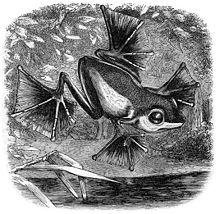
\includegraphics[width = .4\linewidth]{plus-1.jpeg} % 设定图片宽度相对于版心宽度,图片文件资源名
    \caption{华莱士在其著作《马来群岛》中绘制的飞蛙速写} % 图的题注
    \label{fig:plus-1} % 与 autoref 关联,设定交叉引用和显示「图x.x」
\end{figure}


% 梦里不觉 ☐ 已深, ☐ ☐ 岂是为他人。
\subparagraph{华莱士飞蛙} % +1s
华莱士飞蛙 (Rhacophorus nigropalmatus) ,
得名于它的发现者——生物学家阿尔弗雷德 · 华莱士 (Alfred R. Wallace)。
华莱士飞蛙生活在马来半岛的森林里,
它的体型很大,体长有 8 到 10 厘米,
除了交配和产卵,它们几乎从不下树……
如\autoref{fig:plus-1} 所示。

您是否注意到了,
源码中单个换行符并不会被编译成文档中的换行,
而两个或者超过两个换行符将开启一个新段落。
(类似HTML中新建了一个\texttt{<p>}标签)。
如果需要在文章中随意插入一个换行(类似于\texttt{<br>}标签),
则应该在源码文件中编写$\backslash\backslash$实现。
此标记一般仅在排版表格时使用,
或者活用于后期微调工作。

由于\LaTeX 的命令会使用几个固定的字符,
同其他编程语言处理字符串时一样,
当输出此类字符时需要使用逃逸策略,
如果您的论文编译错误,请\textbf{优先检查是否忘记逃逸此类字符}
\footnote{鄙人在写这份文档的时候都还是会忘记记给下划线逃逸(\LaTeX 命令使用下划线表示下标)}。
逃逸规则见\autoref{tab:escape} 所示。


% 和图一样,这里的htbp先不要管,先照抄
\begin{table}[htbp]
    \centering  % 依照规定 表格必须居中版心放置
    \caption{\LaTeX 命令专用字符逃逸规则} % 表格题注,zjuthesis.cls 将其设置在表格之上
    \label{tab:escape} % 交叉引用
    \begin{tabu}{lllllllll} % 9 列均左对齐
        \toprule % 头线
        输出 & \#  & \$  & \&  & \_  & \{   & \}  & \~{}  & \`{} \\ % 注意到了这个换行符吗
        \midrule % 中线
        源码 &  % 感受一下这里的「逃逸」
        \texttt{$\backslash$\#} &
        \texttt{$\backslash$\$} &
        \texttt{$\backslash$\&} &
        \texttt{$\backslash$\_} &
        \texttt{$\backslash$\{} &
        \texttt{$\backslash$\}} &
        \texttt{$\backslash$\~{}} &
        \texttt{$\backslash$\`{}}\\
        \bottomrule % 底线
    \end{tabu}
\end{table}

至于反斜杠本身的逃逸方法,请见上一段文字或表格的源码。

默认情况下,
多个空格符、水平制表符或单个换行符,
都仅会被编译成文档中的一个空格,
然而,和西文不同,中文的词与词之间是没有空格的,
所以本模板在XeCJK环境的初始化配置上取消了此类规则。
利用这样的改动,
您在编写论文时可按照您的行文思路随意换行,
不必担心产生多余的空格。
随着您的行文篇幅渐巨,
您将慢慢体会到这种编辑方式的优势——
\textbf{内容}与\textbf{样式}的分离。

输出英文半角双引号,需要在源码编写两个反引号(``grave'')。
而中文双引号则直接在源码中编写一对全角双引号即可。
鉴于目前大陆地区的官方标准明确规定使用此种方法标记引号,
请不要在论文中使用台湾地区和日本等地使用的直角引号
\footnote{网页中文排版近年来有惯用直角引号的趋势,此处不讨论}。

% 论文除了第一章绪论和终章的总结与展望, 最后都需要撰写一节“本章小结”。
% 活用注释作为 ToDo 提醒是一个好习惯
\section{本章小结}
本章简单描述了\LaTeX 排版的基本概念和本模板的源码结构,
通过同步实例介绍了最基本语义单元的编写。
现在,您可以尝试开始编写自己的论文,
当遇到无法排版的元素或无法解决的问题时,
欢迎继续阅读下一章。

%!TEX root = ../main.tex

\chapter{学位论文排版元素}

通过阅读上一章,
相信您已基本配置完成编辑环境,
以及如何正确编写各级章节和段落,
了解容易引起编译出错的逃逸字符。

如果您仔细阅读过源码,
您应该已经懂得使用命令\texttt{$\backslash$begin\{xxxx\}}开始一段新的布局环境。
现在将稍系统地介绍计算机类学位论文中的排版元素,及其编写方法。
本章主要介绍以下排版元素:
\begin{itemize}
    \item 列表环境(包括有序、无序、定义三种列表)
    \item 插图和表格
    \item 代码环境
    \item 数学和算法环境
\end{itemize}

本章尽量覆盖论文写作中的大部分场景,但不面面俱到。
如有特殊需求,请仔细阅读相关宏包手册或求助于国内外TeX社区及问答网站。

\section{列表环境}

列表环境有三种,
类似与HTML的\texttt{<ol>},
\texttt{<ul>},\texttt{<dl>}
三个标签。
以下是一个定义列表环境:
\begin{description}
    \item[有序列表] enumerate 默认从阿拉伯数字1开始编号\footnote{如需更改请搜索“重定义列表”}
    \item[无序列表] itemize 默认圆点标记,尽量少用
    \item[定义列表] description 语义上用于一系列简短解释
\end{description}

列表可以嵌套,比如:
\begin{enumerate}
	\item 第一级列表
	\item 第一级列表
	\begin{enumerate}
		\item 第二级列表
		\item 第二级列表
        \begin{itemize}
            \item 第三级列表
            \item 第三级列表
		\end{itemize}
		\item 第二级列表
		\item 第二级列表
	\end{enumerate}
\end{enumerate}

\section{插图环境和浮动体}

相信您在上一章的探索学习中已经基本掌握了插入图片的方法,
但可能仍存疑虑。
现在先简单介绍浮动体的概念,
以助您理解插图环境的布局规则,
最后再介绍子图的排布以应对您更高的排版需求。
% 关于绘图,本文将在后续章节讲述
关于图的绘制,本文将在\ref{how-to-plot} 继续讲述。 % 活用ref引用,让评阅老师随处移动

当一个图片或表格太大在当前页面无法继续排版时,
一种简单的解决方案,
即是新开一页排版(Word 默认模式),
前页可能留下大段空白,十分不美观。
\LaTeX 的默认解决方案是把它们“浮动”到下一页,
与此同时将后续正文文本填充到插入点后。

插图和表格在\LaTeX 排版中默认为一个浮动体,
当排版引擎试图放置一个浮动体时,它将遵循以下规则:
\begin{enumerate}
    \item 浮动体的布局大小不得超过版心\footnote{版心是指排版文字和图表的区域,一般在页面的中心。——百度百科},否则不能通过编译(Overfull Page Error)
    \item 浮动体只能向后浮动,无法向前浮动
    \item 浮动体默认按照 h $\to$ t $\to$ b $\to$ p 规则布局
    \begin{description}
        \item[h] 排布在当前位置,如果本页所剩空间不够,忽略,检查规则 t
        \item[t] 浮动到下一页顶部
        \item[b] 浮动到下一页底部(脚注之下)
        \item[p] 浮动到一个允许出现浮动体的页面
        \item[!] 忽略浮动体放置的大多数内部参数\footnote{在下也不太懂}
    \end{description}
    \item 设置 htbp 参数的顺序不会影响默认的规则顺序
\end{enumerate}
在实践中,一般选用浮动规则[htbp], [tbp], [htp], [tp] 来完成浮动体布局。
请不要使用单一参数布局,这样极有可能出现难解的浮动问题。
不适当的浮动规则参数将导致浮动对象被放进一个队列中等待布局,
如果队列中浮动对象超过 18 个,编译时报Too Many Unprocessed Floats错误。
当需要在一页中排版的图片较多时,
您可以通过\texttt{$\backslash$clearpage}命令强制在此处排版完所有浮动体
后在排版其他内容。关于清除浮动等复杂主题,此处不再展开。

一般实践中,插图尺寸不宜超过版心一半,插图也不宜过密。
另外,可以在论文内容稳定后,
通过前置插图代码,
强行“向前浮动”,保证插图和引用处的距离不至于太远。
% 破坏语义,不宜滥用

关于本模板对浮动体的设置,参看\texttt{zjuthesis.cls},
搜索关键字“浮动体”找到对应配置。
图片引用路径在\texttt{zjuthesis.cls}里定义的\texttt{graphicspath}里,
默认情况下,\texttt{$\backslash$includegraphics}命令从论文源码根目录搜索,
如果在根目录里找到文件,则不再继续往定义引用路径搜索,
当引擎无法找到您指定的图片资源时,会导致编译错误。
注意,引用的文件名包括文件后缀。

% 现在你可以随意更动此插图代码的位置来感受一下浮动体布局的规则
\begin{figure}[htbp]
	\centering
	\begin{subfigure}[b]{.45\textwidth}  % 注意此处的尺寸控制
		\centering
		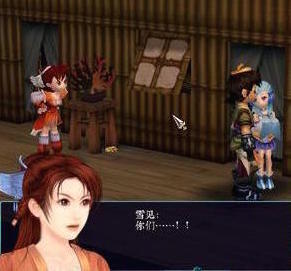
\includegraphics[width = \textwidth]{xuejian.jpg}
		\caption{仙三}\label{fig:subfig-samp1}
	\end{subfigure}
	\begin{subfigure}[b]{.45\textwidth}
		\centering
		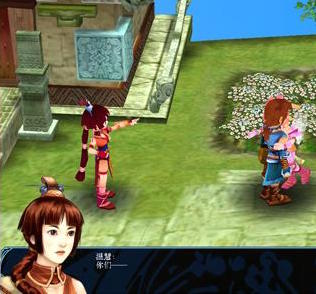
\includegraphics[width = \textwidth]{wenhui.jpg}
		\caption{仙三外}\label{fig:subfig-samp2}
	\end{subfigure}
	\begin{subfigure}[b]{.45\textwidth}
		\centering
		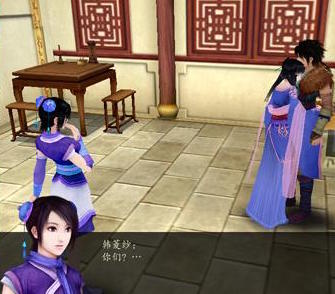
\includegraphics[width = \textwidth]{lingsha.jpg}
		\caption{仙四}\label{fig:subfig-samp3}
	\end{subfigure}
	\caption{仙剑白学传}\label{fig:subfig-samp}
\end{figure}

接下来描述子图的编写,
在实际论文撰写过程中,
经常需要比较几组实验数据或场景。
此时,合乎语义的做法是为不同的组设置子图,
而不是分别设图。

多个子图组成一个单独的浮动体布局,
共用一个总图题和总引用,并可以有各自单独的子图题和引用。
本模板使用subcaption 宏包处理子图排版,如\autoref{fig:subfig-samp} 所示
论文中不可像本文一般,
平白无故地出现与行文毫无关联的图例,
而且,必须有适当的文字内容对图例做出解释。
比如,比较分析从\autoref{fig:subfig-samp1} 到\autoref{fig:subfig-samp3}
仙剑系列在白学梗方面的运用变迁。\footnote{往后数代仍有类似场景 -\_-\# (顔文字書込禁止!)}

当准备插图资源时,应该尽可能保证插图清晰,背景透明。
图中文字大小应与文中接近,不小于脚注文字大小,不大于正文段落文字大小,
框线宽度不大于2px。

如果您曾关注过图片的格式,
应该知道图片在计算机中一般分为矢量图(\autoref{fig:vector})和位图(\autoref{fig:raster})两种类型。
通俗地说,矢量图通过几何属性存储图片信息,
所以能在缩放时保持图形的几何属性。
而位图按像素点存储图片信息,在缩放时必然会丢失信息。
对于学位论文里的图例,请尽量使用矢量图,
以给评阅老师或后人精确地参考和还原实验。
常用的矢量图格式有eps, pdf, svg 和 Adobe 系列的文件格式。
其中\LaTeX 格式可以直接引用eps 和 pdf 格式的图片。

\begin{figure}[htbp]
	\centering
	\begin{subfigure}[b]{.45\textwidth}
		\centering
		
\includegraphics[width = \textwidth]{vector.pdf}
		\caption{矢量图}\label{fig:vector}
	\end{subfigure}
	\begin{subfigure}[b]{.45\textwidth}
		\centering
		
\includegraphics[width = \textwidth]{raster.png}
		\caption{位图}\label{fig:raster}
	\end{subfigure}
	\caption{Google Logo 的矢量图和位图比较}\label{fig:vector-raster}
\end{figure}


\section{表格}
表格与插图一样,也是浮动体单位。
在\LaTeX 中,表格的编写成本比较高,
极易引发编译错误。
初期建议同学们直接复制本模板表格进行修改。
对于只有两列的表格,建议改用列表环境完成排版。
本模板使用tabu排版表格,
使用longtabu排版超长表格。
学术论文多用线条简洁的三线表,
所谓三线就是 toprule, midrule和bottomrule 。
如\autoref{tab:tabu_test_1} 是对tabu宏包的tabu表格环境测试。
\begin{table}[htbp]
	\centering
	\caption{这是一个用tabu环境的测试用的表格}\label{tab:tabu_test_1}
    \begin{tabu}{lrr} % lrr 表示 左对齐 右对齐 右对齐
    %\begin{tabu}{|l|r|r|} % 加上竖线看看

    \toprule % 软件学院论文模板规定表头必须加粗
    \textbf{行星}     & \textbf{赤道半径}km & \textbf{公转周期}d \\
    \midrule
    水星     & 2.439  & 87.9 \\
    金星     & 6.1    & 224.682 \\
    地球     & 6378.14 & 365.24 \\
    \bottomrule
    \end{tabu}%
\end{table}

\autoref{tab:tabu_test_2} 对tabu to表格的x列模式进行测试。在表格导言区中设置为X[1]X[2]X[2],表示这三列表格的列宽比值为1:2:2,总的表格宽度由tabu to环境设置,这里设置为0.6\textbackslash linewidth。相比于tabular环境,tabu环境的列宽设置方便许多。
\begin{table}[htbp]
	\centering
	\caption{tabu环境测试表格---X列模式}\label{tab:tabu_test_2}
    \begin{tabu} to 0.6\linewidth{X[1]X[2]X[2]}
    \toprule
    \textbf{行星}     & \textbf{赤道半径}km & \textbf{公转周期}d \\  % 为了表格排版的美观 表头建议加粗
    \midrule
    水星     & 2.439  & 87.9 \\
    金星     & 6.1    & 224.682 \\
    地球     & 6378.14 & 365.24 \\
    \bottomrule
    \end{tabu}%
\end{table}

如\autoref{tab:tabu_test_3}是longtabu环境测试表格。
longtabu环境不能用在table浮动体环境中。
根据GB/T 7713.1-2006规定:如果某个表需要转页接排,
在随后的各页上应重复表的编号。
编号后跟标题(可省略)和“(续)”, % 表:「我要续…… +1
置于表上方。
续表应重复表头。

特别需要注意的是,
longtabu是基于longtable宏包开发的,
所以在zjuthesis.cls文件中已经插入了longtable宏包。
longtable环境的所有功能都可以在longtabu中使用,
如\textbackslash endhead,
\textbackslash endfirsthead,
\textbackslash endfoot,
\textbackslash endlastfoot,
和\textbackslash caption等。
具体用法请参见longtable和tabu宏包的相应文档。

\begin{longtabu}{lccc}
\caption{材料弹性模量及泊松比}\label{tab:tabu_test_3}\\
\toprule
名  称   & 弹性模量E/Gpa & 切变模量G/Gpa & 泊松比$\mu$ \\
\midrule%
\endfirsthead
\caption{材料弹性模量及泊松比(续)}\\
\toprule
名  称   & 弹性模量E/Gpa & 切变模量G/Gpa & 泊松比$\mu$ \\
\midrule%
\endhead
\bottomrule%
\endfoot
镍铬钢、合金钢 & 206    & 79.38  & 0.3 \\
碳 钢    &  196~206 & 79     & 0.3 \\
铸 钢    &  172~202 &        & 0.3 \\
球墨铸铁   &  140~154 &  73~76 & 0.3 \\
灰铸铁、白口铸铁 &  113~157 & 44     &  0.23~0.27 \\
冷拔纯铜   & 127    & 48     &   \\
轧制磷青铜  & 113    & 41     &  0.32~0.35 \\
轧制纯铜   & 108    & 39     &  0.31~0.34 \\
轧制锰青铜  & 108    & 39     & 0.35 \\
铸铝青铜   & 103    & 41     & 0.3 \\
冷拔黄铜   &  89~97 &  34~36 &  0.32~0.42 \\
轧制锌    & 82     & 31     & 0.27 \\
硬铝合金   & 70     & 26     & 0.3 \\
轧制铝    & 68     &  25~26 &  0.32~0.36 \\
铅      & 17     & 7      & 0.42 \\
玻璃     & 55     & 22     & 0.25 \\
混凝土    &  14~39 &  439~15.7 &  0.1~0.18 \\
纵纹木材   &  9.8~12 & 0.5    &   \\
横纹木材   &  0.5~0.98 &  0.44~0.64 &   \\
橡胶     & 0.00784 &        & 0.47 \\
电木     &  1.96~2.94 &  0.69~2.06 &  0.35~0.38 \\
赛璐珞    &  1.71~1.89 &  0.69~0.98 & 0.4 \\
可锻铸铁   & 152    &        &  \\
拔制铝线   & 69     &        &  \\
大理石    & 55     &        &  \\
花岗石    & 48     &        &  \\
石灰石    & 41     &        &  \\
尼龙1010 & 1.07   &        &  \\
夹布酚醛塑料 &  4~8.8 &        &  \\
石棉酚醛塑料 & 1.3    &        &  \\
高压聚乙烯  &  0.15~0.25 &        &  \\
低压聚乙烯  &  0.49~0.78 &        &  \\
聚丙烯    &  1.32~1.42 &        &  \\
硬聚氯乙烯  &  3.14~3.92 &        &  \\
聚四氟乙烯  &  1.14~1.42 &        &  \\
\end{longtabu}%


\section{代码段}

原则上,论文中应尽可能少的出现工程代码。
如果您必须引用一小段代码,
可以使用\texttt{lstlisting}设置代码环境。
本模板的代码环境默认配置在\texttt{zjuthesis.cls},
您可以搜索关键字“代码”找到配置。

本模板不鼓励引用大段代码,
所以默认情况下不为代码环境开启行号功能。
观察\autoref{code:samp-code},结合前述图表设置,
试图理解代码环境的编写。

\begin{lstlisting}[language=C++,numbers=left, numberstyle=\tiny,label=code:samp-code, caption=一段Chromium的源代码]
// Start tasks to take all the threads and block them.
  const int kNumBlockTasks = static_cast<int>(kNumWorkerThreads);
  for (int i = 0; i < kNumBlockTasks; ++i) {
    EXPECT_TRUE(pool()->PostWorkerTask(
        FROM_HERE,
        base::Bind(&TestTracker::BlockTask, tracker(), i, &blocker)));
  }
  tracker()->WaitUntilTasksBlocked(kNumWorkerThreads);

  // Setup to open the floodgates from within Shutdown().
  SetWillWaitForShutdownCallback(
      base::Bind(&TestTracker::PostBlockingTaskThenUnblockThreads,
                 scoped_refptr<TestTracker>(tracker()), pool(), &blocker,
                 kNumWorkerThreads));
  pool()->Shutdown(kNumWorkerThreads + 1);

  // Ensure that the correct number of tasks actually got run.
  tracker()->WaitUntilTasksComplete(static_cast<size_t>(kNumWorkerThreads + 1));
  tracker()->ClearCompleteSequence();
\end{lstlisting}

引用一两行代码,可以直接使用\texttt{verbatim}环境完成。
注意,此环境不会采取任何主动断行策略。
\begin{verbatim}
Error: Command failed: /bin/sh -c rsync -arvq --exclude cache
--exclude .git 
\end{verbatim}

\section{数学和算法环境}

\TeX 模板引擎创立之初就是为了更美观地排版数学公式。
在理工科的学位论文中,数学符号和数学公式必不可少
\footnote{至于定理、引理和推论等纯理科环境,本模板未作任何设定,不讨论。}。
在本模板中,数学环境由amsmath和amssymb宏包支持。
(即便没有使用公式,您应该也希望看到$a_1$, $a_2$, $C_n^m$而不是a1, a2, Cnm 吧?)

简单的行内公式,
直接在源码处编写\texttt{\$...\$}内的公式即可,
不熟习\LaTeX 公式编写的同学,
可以使用可视化的公式编辑器产生\LaTeX 代码,
这里推荐使用Daum Equation Editor完成复杂公式编辑的工作。

对于单行公式,可以使用\texttt{\$\$...\$\$}创建。
$$Y=\sum_{k=1}^n X_k$$
如果需要设定交叉引用,推荐align环境创建,如\eqref{eq:samp}所示。
\begin{align}\label{eq:samp}
    f(x) & = 2(x + 1)^{2} - 1\\                  % & 用来对齐等号
		 & = 2(x^{2} + 2x +1)-1\\
		 & = 2x^{2} + 4x + 1
\end{align}

%一个矩阵
%$$\begin{bmatrix}
%1&2&3&4\\
%5&6&7&8\\
%9&10&11&12
%\end{bmatrix}$$

计算机类的学位论文
一般少不了对研究算法的描述。
本模板选用algorithmi2e宏包排版算法环境。
详细指令使用方式参见宏包使用手册
\footnote{一般有需求排布复杂算法的同学应该有一定的科研经历}。
如\autoref{algo:duplicate2}

\begin{algorithm}
\DontPrintSemicolon
\KwIn{A sequence of integers $\langle a_1, a_2, \ldots, a_n \rangle$}
\KwOut{The index of first location with the same value as in a previous location in the sequence}
$location \gets 0$\;
$i \gets 2$\;
\While{$i \leq n \land location = 0$} {
  $j \gets 1$\;
  \While{$j < i \land location = 0$} {
    % The "l" before the If makes it so it does not expand to a second line
    \lIf{$a_i = a_j$} {
      $location \gets i$\;
    }
    \lElse{
      $j \gets j + 1$\;
    }
  }
  $i \gets i + 1$\;
}
\Return{location}\;
\caption{{\sc FindDuplicate2}}
\label{algo:duplicate2}
\end{algorithm}

\section{绘图}\label{how-to-plot}

一图胜千言,经过同学们辛苦的实验积累下的数据,
相比于冗长的文字描述,
绘图呈现的信息结构将更具可读性。
使用强大的TikZ宏包,可以绘制各式各样的图例,
比如在\ref{dirtree} 的目录结构图就是使用TikZ宏包绘制完成。
通过绘图宏包得到的是矢量图,
经过缩放后仍能精确地指导打印。
遗憾的是,
由于使用TikZ宏包绘制图例的方法艰深繁杂,
非长期钻研学术者实不可速取。

% 这里删掉了一大段TikZ宏包的使用
% 太复杂了  如果不是跟老师搞学术的话真的算了

含有大量数据的统计图,
从事数据分析工作的同学可自行使用python或R语言完成绘制,
确保输出eps或pdf格式图形,使用插图环境引入即可。

对于一般的流程图,本模板推荐使用graphviz绘图工具绘制。
相对于TikZ,graphviz已经足够适合人类掌握了。
如果坚持使用可视化工具完成此类图例的绘制,
本文推荐一个在线绘图工具\texttt{https://www.draw.io}\footnote{请保证科学上网。},
该工具可以绘制流程图、UML图、实体关系图。
另外它还支持 Dropbox 同步及输出 pdf,
通过同步论文的图片引用目录,
可以最高效的完成绘图和插图的工作。

无论用何种工具完成,
时间精力成本都不会太低。
请妥善规划您的论文撰写时间,
确保顺利毕业。

\section{关于参考文献}

硕士学位论文的参考文献,
请严格按照导师和学院规定,
注重引文质量,万不可滥引。

参考文献参照国家标准《GB/T 7714-2005: 文后参考文献著录规则》
\footnote{此标准规定的学位论文引用格式并无指定需列出是“硕士学位论文”还是“博士学位论文”},
样式文件由南京大学胡海星提供。
\begin{verbatim}
http://haixing-hu.github.io/nju-thesis/
\end{verbatim}

学校规定,参考文献采用顺序编码制,
即引文处采用序号标注,参考文献表按引文序号顺序列出。
参考文献的排版需要引入同学们自己的文献数据库,
南京大学胡海星提供了一个样例数据库,见其代码仓库内\texttt{references/test.bib}。
通过各式文献管理工具(如Zotero),您可以在论文早期工作时逐渐积累文献数据库。
通过Google学术查找一篇文献时,如\autoref{fig:gscholar} 所示,点击cite,
选择BibTeX,即可得到本文献的Bib格式的各项字段。
\begin{figure}[htbp]
    \centering
    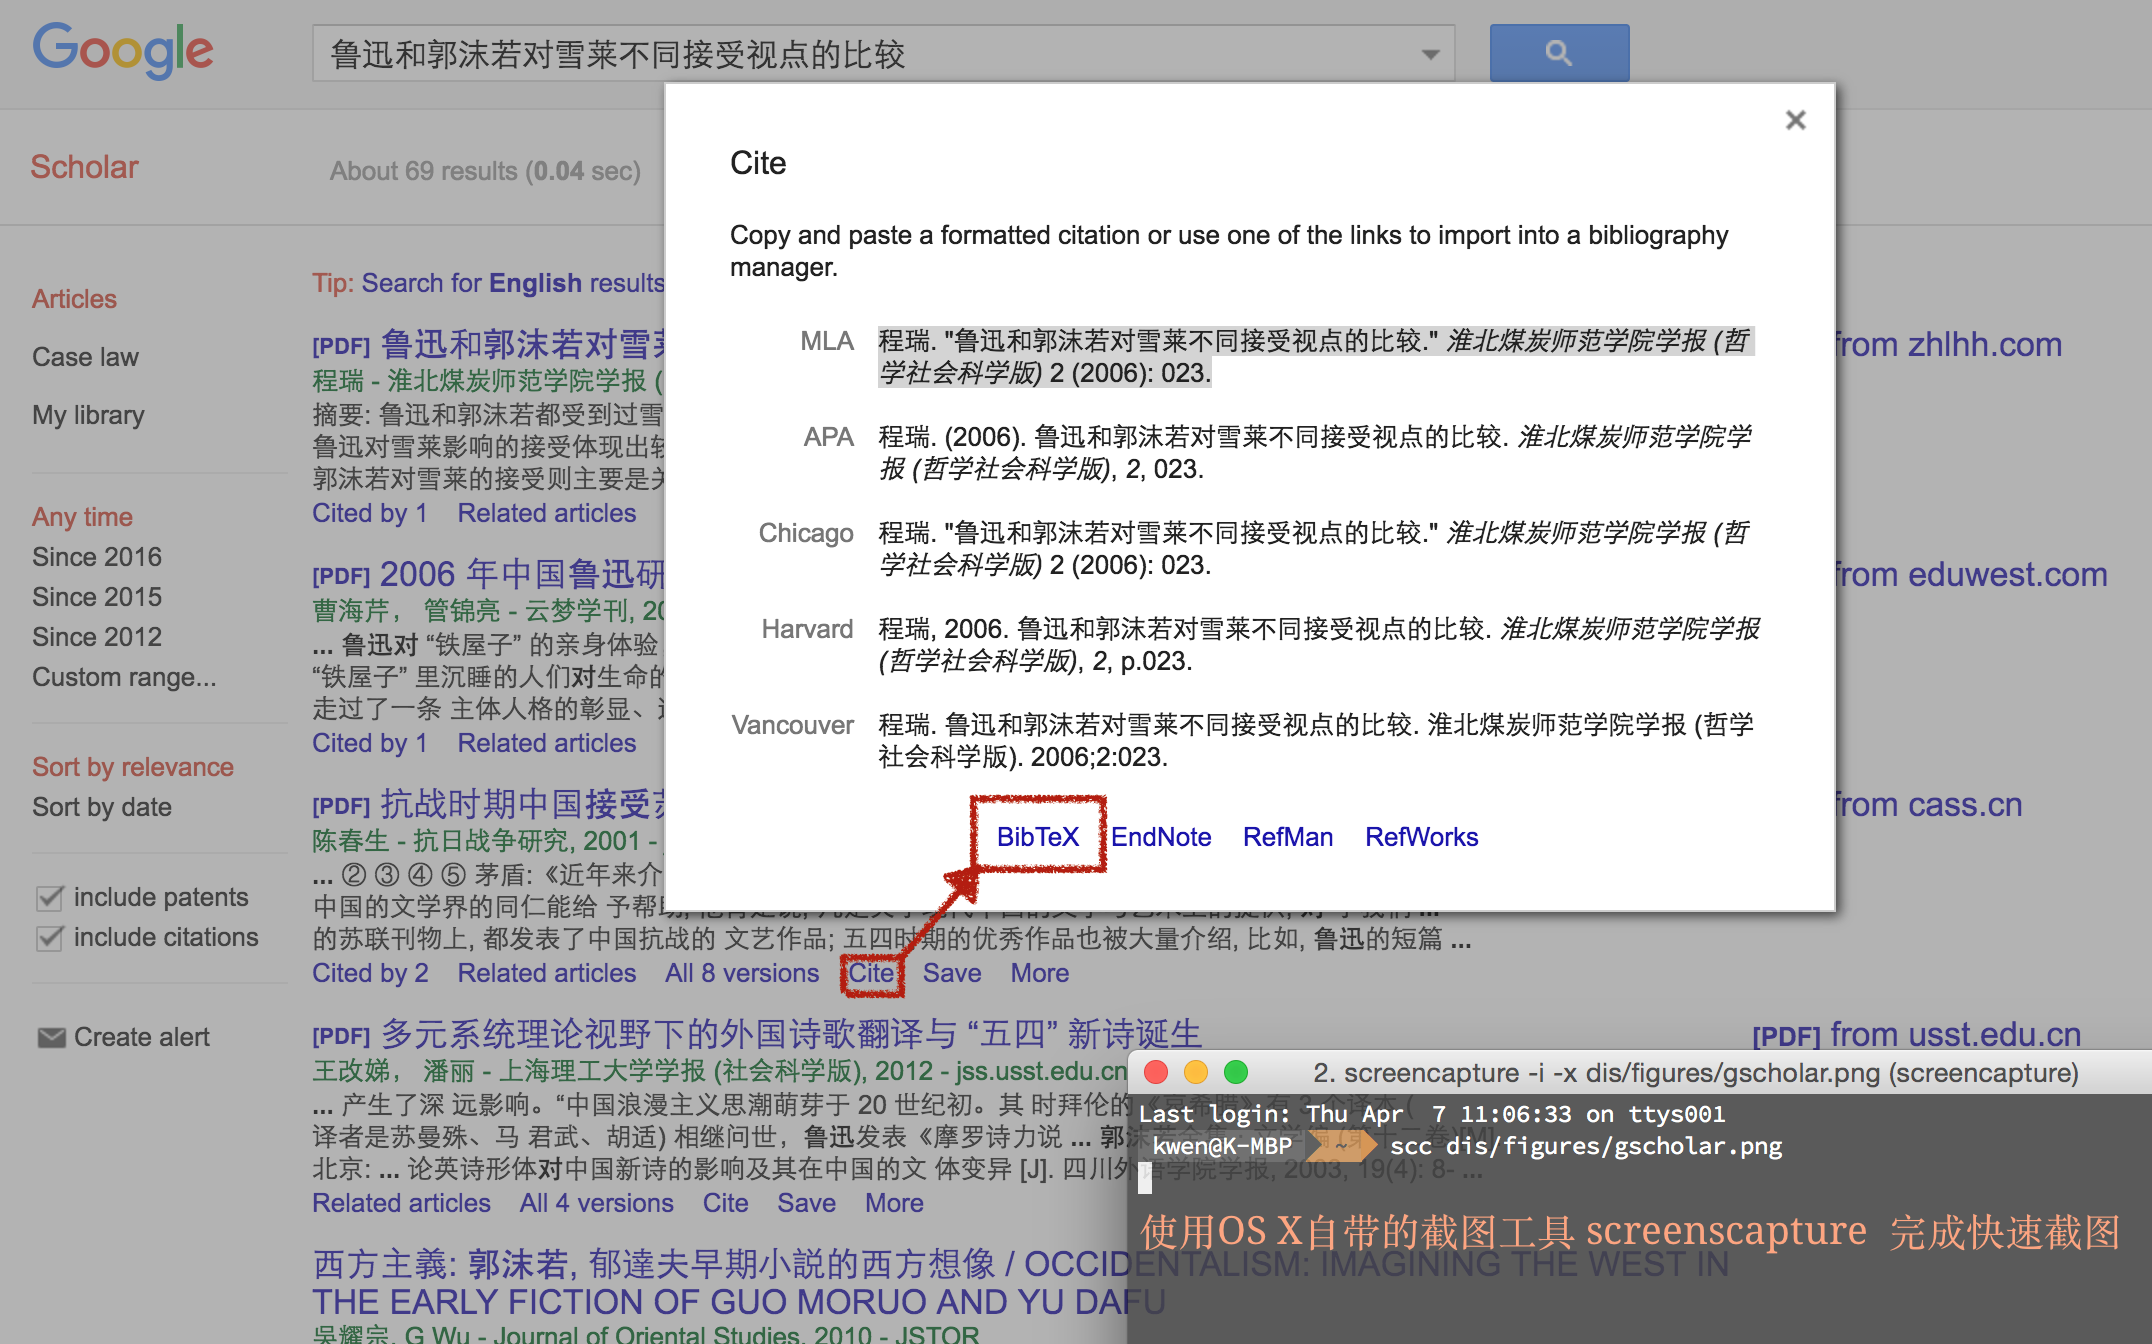
\includegraphics[width=\textwidth]{gscholar.png}
    \caption{使用Google学术查找引文的BibTeX字段}
    \label{fig:gscholar}
\end{figure}

由Google学术提供的文献类型和字段有可能不满足胡海星前辈的设定,
注意调整。
以下是常用的文献类型:
\begin{description}
    \item[期刊]          \texttt{@article}
    \item[专著]          \texttt{@book, @inbook}
    \item[译著]          \texttt{@Book, @inBook}
    \item[会议论文集]    \texttt{@proceeding, @inproceeding}
    \item[手册]          \texttt{@manual}
    \item[网页]          \texttt{@webpage, @online}
\end{description}

\begin{itemize}
    \item 比如这是一篇中文期刊\cite{lixiaodong1999}
    \item 这是几篇英文期刊\cite{christine1998, kanamori1998}
    \item 一本中文书\cite{zh-book-1}
    \item 一本中文译著\cite{anwen1988b}
    \item 一本英文书\cite{lamport1994latex, takeuti1973}
    \item 一篇中文inproceeding\cite{nonlinear1996}
    \item 中文proceeding\cite{a2-1}
    \item 英文proceeding\cite{a2-2}
    \item 中文inproceeding\cite{aczel1998}
    \item 一篇学位论文\cite{a4-1} 
    \item 其他资料:手册\cite{ipad}报纸\cite{renminribao}网页\cite{dubash2010}
\end{itemize}

在论文中设置了一个错误或丢失的引用不会引起编译错误,
引擎会在引用标记中设一个问号。
手动编译论文的顺序一般为:
\begin{verbatim}
xelatex main
bibtex main  // 生成参考文献
xelatex main
xelatex main
\end{verbatim}
而latexmk 自动化地执行了这些步骤,所以编译时间才需要20余秒之久。







\section{本章小结}

本章划分节比较多,正式行文中请尽量避免。

传播智识,单单借助文字的力量是无力的,
即使是日常博客文章,列表、插图、表格、代码都少不了。
何况是一篇用于申请硕士学位的论文呢?

一篇学位论文集长期的科研工程实践智慧于寥寥数万字。
如何合理规划论文语义和排版元素,
让即便不熟习此领域的后人能在短时间内消化,
得以继续开物前民,
是一个值得反复求索的话题。


%!TEX root = ../main.tex

\chapter{总结和展望}

\section{相关工作总结}

本模板主要内容来源于ZJU-Awesome项目,
参考软件学院论文格式要求做出调整,
并加入补充宏包,调整若干属性配置完成。
封面方面主要调整了各栏间距和对齐,
摘要依照软件学院更改了关键字的样式和页码的样式。
软件学院规定从摘要起每页必须有对应章标题的页眉,
虽然在一般排版习惯里,章头处不应设置页眉,
但考虑到已有大部分同学使用Word字处理软件遵照执行,
为保一致性,本模板暂时向软件学院的设定妥协。
由于论文格式要求并未向章头处的间距做出任何设定,
本模板保留ZJU-Awesome设定。
除此之外,本模板还做出了不少微小的改动。
详情请仔细阅读\texttt{zjuthesis.cls}和\texttt{main.tex}相关内容。

考虑到大部分软件学院的同学对\LaTeX 论文排版的陌生,
本文以尽量精炼的篇幅介绍了论文排版工作的各方面。
现在给出一个参考流程如\autoref{fig:workflow} 希望能对初次使用
\LaTeX 排版论文的同学一点提示。

\begin{figure}[htbp]
    \centering
    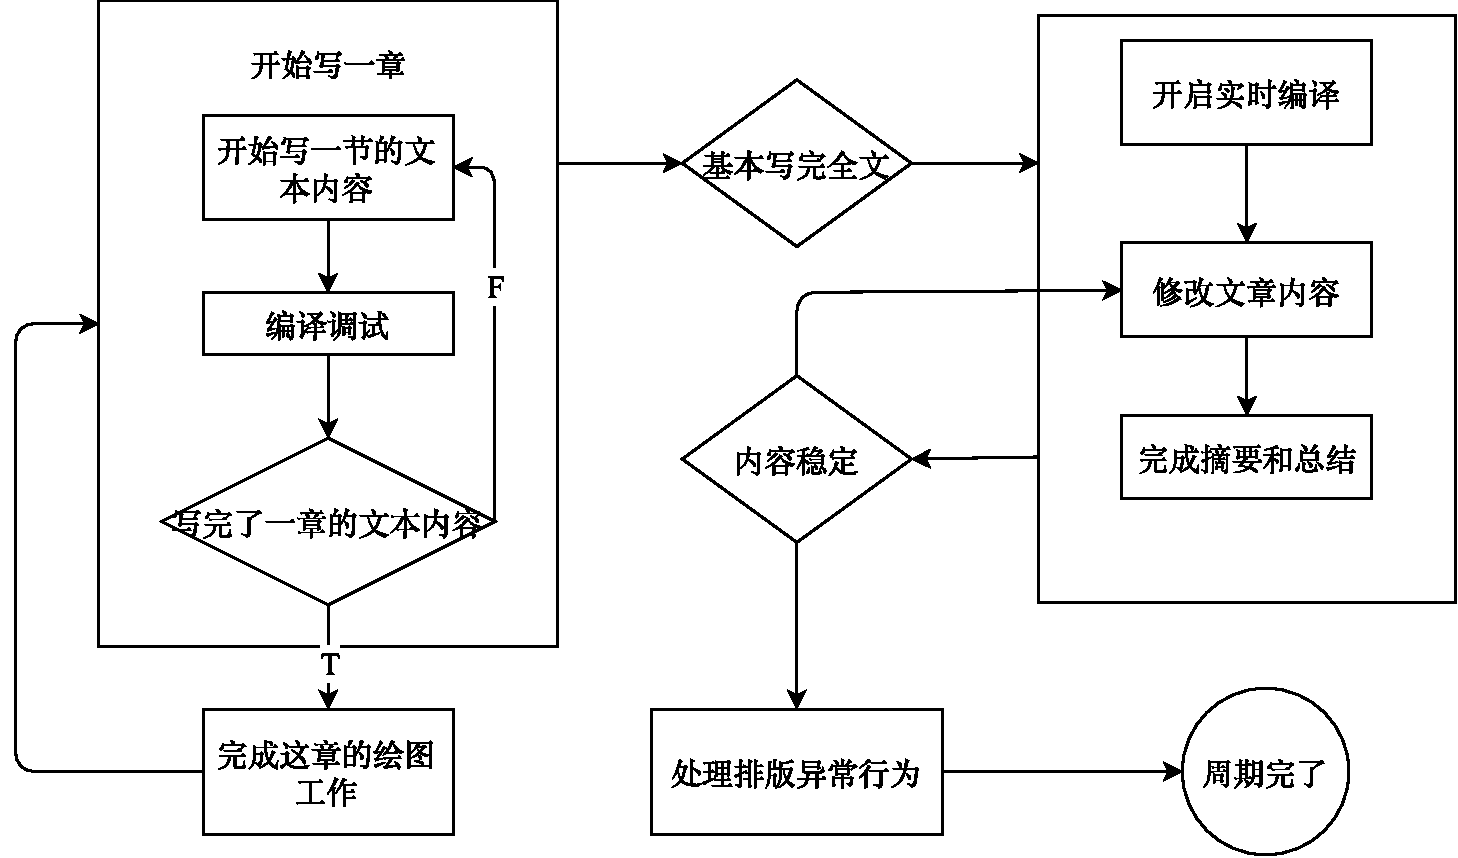
\includegraphics[width=.8\textwidth]{workflow.pdf}
    \caption{论文排版工作参考流程}
    \label{fig:workflow}
\end{figure}

\section{展望}

本文没有讨论各式\LaTeX 环境的使用细则,宏包的具体细节,
调试查错的技巧,也几乎没有交待任何一种具体的绘图方案。
希望屏幕前的你能以最少的代价完成论文排版工作,
养成内容和样式分离的电子写作习惯,
并能独立思考信息表达的最佳模式。

本文草拟于2016年夏季毕业论文送审前,
希望本文能抛砖引玉,
对\LaTeX 有经验的后辈们若能继续完善甚至颠覆本模板的设定,
相信一定能对软件学院的论文排版素质起到根本的改善作用。

\section{真实参考资料}

考虑到下一页的参考文献是样例凑数,
此处不完整且不严谨地列出本文真实的参考资料:
\begin{description}
    \item[常规文档] \texttt{http://latexfly.com/docs/}
    \item[算法宏包] \texttt{https://en.wikibooks.org/wiki/LaTeX/Algorithms}
    \item[参考文献管理] \texttt{https://www.zhihu.com/question/23565739}
    \item[优雅的使用Word] \texttt{https://www.zhihu.com/question/20541531}
    \item[电子科大论文模板] \texttt{https://github.com/shifujun/UESTCthesis/wiki}
    \item[实时编译] \texttt{http://xiaoweiz.github.io/posts/2014/Aug/ST\_skim\_latexmk/}
    \item[一份不太简短的\LaTeX2e 介绍]   
    \item[各种宏包的手册] 在 TeX Live Utility 就可以查看
\end{description}
  % 总结和展望

% 结尾部分排版
\backmatter

% 引用参考文献数据库
\bibliography{references/test.bib}

% 附录部分
%\appendix
%\include{contents/appendixA}

% 作者简历
% !TEX root = ../main.tex
\chapter{作者简历}
\noindent 教育经历:

\begin{tabular}{llll}
    2014年9月至2016年6月: &  浙江大学  & 软件工程  &  硕士    \\
    2010年9月至2014年6月: &  三墩工学院  & 电脑挖掘机维修  &  混混
\end{tabular}

\noindent 工作经历:

\begin{tabular}{llll}
    2015年6月至2016年3月: &  FLAG   &  码畜
\end{tabular}

% \noindent 攻读学位期间发表的论文或研究成果:



% 致谢
% 致谢不必感谢在下,
% 但请一定感谢清华大学薛瑞尼、
% 机械工程学院陈九历
% !TEX root = ../main.tex
\chapter{致\ZJUspace{}谢}

在去年撰写开题报告和文献综述时,
搜索Github发现了仅在数月前发布的ZJU-Awesome项目。
简单套用后自觉此法应当推广。
于是在2016年3月撰写论文结束后,
下决心向软件学院的同学推广此一模板,
继而有了本文和在下对模板的调整。

衷心感谢ZJU-Awesome项目作者之一机械工程学院的陈九历同学耐心解答在下的多次疑问。

% 难道不应该感谢世界(大雾)
也感谢夏目友人帐能让我在论文写作过程中保持着一份平静,
最后感谢这份文稿前的你,能仔细阅读到这一页。

\vspace{2cm}
\hfill
\begin{minipage}{14em}
    \begin{flushright}
        君之名\\
        %于浙江大学软件学院\\ % 学院要求的格式 - -#
        %2016年4月18日   % 与封面论文提交时间一致
        2017年1月1日\\
        于老和山下
    \end{flushright}
\end{minipage}


\end{document}
